\documentclass[11pt]{article}

% --- Packages ---
\usepackage[utf8]{inputenc}
\usepackage[T1]{fontenc}
\usepackage{times}
\usepackage{graphicx}
\usepackage{amsmath,amssymb}
\usepackage{booktabs}
\usepackage[margin=1in]{geometry}
\usepackage{xcolor}
\usepackage{hyperref}
\usepackage{multirow}
\usepackage{colortbl}
\usepackage{enumitem}
\usepackage{caption}
\usepackage{subcaption}

% --- Page setup ---
\pagestyle{plain}
\graphicspath{{./figures/}}

% --- Custom commands ---
\newcommand{\RRE}{RRE}
\newcommand{\CFR}{\text{CFR}}
\newcommand{\AURC}{\text{AURC}}
\newcommand{\RPC}{R_{\text{PC}}}

% --- Title ---
\title{\Large\bf When References Disagree:\\Prediction Consistency for Selective Visual Prompting}

\author{Anonymous Authors\\[2pt]
\texttt{\{anonymous\}@anonymous.edu}}

\date{}

\begin{document}
\maketitle

% ======================================================================
\begin{abstract}
Multi-reference visual prompting, where a segmentation model conditions on a query image and 
multiple reference image-mask pairs, has emerged as a flexible paradigm for few-shot segmentation. 
However, different references can produce substantially different predictions for the same query, 
creating a reliability problem: when should we trust the model's output? We formalize this as 
\textit{Reference Reliability Estimation} (\RRE{})---the task of predicting query-level segmentation 
quality without access to query ground truth---and introduce a reference-resampling evaluation 
protocol that isolates the effect of reference choice.

We propose \textit{Prediction Consistency}, a simple, ground-truth-free risk score defined as the mean 
pairwise IoU among segmentations produced by different references. Queries with low prediction 
consistency (high disagreement) are flagged as high-risk and can be selectively abstained, 
enabling coverage-based reliability control. Across five pipelines spanning DINOv2 and SAM/SAM2 
backbones on 80 nuclei segmentation queries, prediction consistency achieves an AURC of 0.0158 
with 88.6\% relative reduction in catastrophic failure rate at 80\% coverage, substantially 
outperforming entropy-based (AURC 0.1281), candidate Jaccard, and prompt overlap baselines. 

Cross-dataset evaluation on MoNuSeg and IDRID reveals boundary conditions: the risk signal 
transfers to datasets where segmentation quality is moderate ($\rho$=0.83 on MoNuSeg), but 
segmentation quality itself may not improve. We conduct systematic ablation of reference count, 
consistency metrics, and pipeline components, and provide an honest analysis of failure modes 
and limitations. This work establishes prediction consistency as a practical approach to 
reliability estimation in multi-reference visual prompting.

\vspace{4pt}
\noindent\textit{Note: This is an exploratory/benchmark paper. No confirmatory holdout cohort was available at the time of writing.}
\end{abstract}

% ======================================================================
\section{Introduction}

Visual prompting has emerged as a powerful paradigm for adapting foundation segmentation 
models to specific tasks without fine-tuning. A typical multi-reference visual prompting 
pipeline uses a visual matcher (e.g., DINOv2) to retrieve similar reference image-mask pairs 
from a support set, then prompts a segmenter (e.g., SAM) with the reference mask locations 
to segment the query image. This approach has been applied to medical image segmentation, 
natural image segmentation, and beyond.

However, a critical reliability issue arises in multi-reference prompting: different reference 
images can produce substantially different segmentations for the same query. Some references 
lead to accurate masks while others produce catastrophic failures. Currently, there is no 
principled way to determine, at inference time, whether a given query's segmentation is 
trustworthy---without access to query ground truth.

We formalize this as \textit{Reference Reliability Estimation} (\RRE{}): given a query image 
and a set of reference image-mask pairs, predict the segmentation quality for the query 
\textit{without} access to the query's ground truth mask. This is a selective prediction 
problem: we want to identify high-risk queries and either flag them for human review or 
abstain from providing a prediction.

Our key insight is simple: when multiple references produce consistent segmentations for a 
query, the result is likely reliable; when they disagree substantially, the result is likely 
unreliable. This intuition leads to \textit{Prediction Consistency}---a risk score computed 
as the mean pairwise IoU among the segmentations produced by different references:

\begin{equation}
\RPC(q) = 1 - \frac{2}{m(m-1)} \sum_{i<j} \text{IoU}(\hat{M}_{q,i}, \hat{M}_{q,j})
\label{eq:pc}
\end{equation}

Because these segmentations are already generated during standard multi-reference inference, 
prediction consistency incurs no additional model calls and requires no query ground truth.

On our primary pipeline (DINOv2-L + SAM-B) with 80 MoNuSAC nuclei segmentation queries, 
prediction consistency reduces the catastrophic failure rate (Dice $<$ 0.1) by 88.6\% at 
80\% coverage (CFR@80 = 0.016 vs.\ baseline 0.154). Cross-pipeline evaluation across five 
pipelines shows directional support in all five, with the strongest effects in SAM-B-based 
pipelines. Cross-dataset evaluation on MoNuSeg reveals that the risk signal transfers 
($\rho$=0.83) but the segmentation quality is dataset-dependent.

Our contributions are threefold: (1) We formalize the \RRE{} problem and introduce a 
reference-resampling evaluation protocol; (2) We propose Prediction Consistency, a simple, 
GT-free risk signal requiring no additional training; (3) We conduct systematic evaluation 
across five pipelines and three datasets with honest boundary analysis.

% ======================================================================
\section{Related Work}

\subsection{Visual Prompting for Segmentation}
Visual prompting leverages foundation models like SAM for downstream segmentation tasks 
by providing visual cues such as points, boxes, or masks. In multi-reference settings, 
a visual matcher retrieves similar reference image-mask pairs, and the segmenter is 
prompted with the reference mask locations. This paradigm has been adopted in medical 
imaging, natural image segmentation, and video object segmentation. However, existing 
work primarily focuses on improving segmentation accuracy through better matching or 
prompt engineering. The reliability of the resulting segmentations---particularly the 
variability introduced by reference choice---has received limited attention.

\subsection{Selective Prediction and Uncertainty Estimation}
Selective prediction allows models to abstain from predictions when confidence is low. 
In segmentation, uncertainty estimation methods include Monte Carlo dropout, ensemble 
disagreement, and test-time augmentation. Most existing approaches require either model 
modification, multiple forward passes, or access to training data for calibration. Our 
work differs in two key aspects: we focus on the \textit{reference-induced} uncertainty 
specific to multi-reference prompting, and our risk signal requires no model modification 
or additional training.

\subsection{Multi-Reference Segmentation}
Few-shot segmentation methods typically use a single or small number of support images. 
Recent work has explored using multiple supports through attention mechanisms or prototype 
learning. Our reference-resampling protocol provides a systematic way to evaluate how 
reference choice affects segmentation quality, and our prediction consistency score 
leverages the multi-reference setup for reliability estimation.

% ======================================================================
\section{Problem Formulation}

\subsection{Reference Reliability Estimation (\RRE{})}
Given a query image $I_q$, a support set of reference image-mask pairs 
$\mathcal{R} = \{(I_r^{(i)}, M_r^{(i)})\}_{i=1}^{N}$, a visual matcher $\Phi$, and a 
segmenter $\Psi$, the multi-reference visual prompting pipeline produces a set of candidate 
segmentations. For each reference $r_i$, the pipeline matches $I_q$ to $I_r^{(i)}$ using 
$\Phi$ and segments $I_q$ using $\Psi$ with the prompt from $r_i$, producing $\hat{M}_{q,i}$.

The \RRE{} task is to predict the segmentation quality $\text{Dice}(\hat{M}_q, M_q^{\text{GT}})$ 
for the query \textit{without} access to $M_q^{\text{GT}}$.

\subsection{Reference-Resampling Evaluation}
To isolate the effect of reference choice, we sample $m$ references from the support set 
and compute $m$ segmentations for each query. The protocol evaluates within-query variability, 
best-worst gap, and catastrophic failure rate.

\subsection{Prediction Consistency}
For a query $q$ with $m$ references producing segmentations $\hat{M}_{q,1}, \ldots, \hat{M}_{q,m}$, 
the risk score is defined in Eq.~\ref{eq:pc}. Higher $\RPC(q)$ indicates lower agreement 
among references and thus higher predicted risk.

\subsection{Coverage-Based Selective Prediction}
Given a risk ranking of queries, we define a coverage level $c \in (0, 1]$ as the fraction 
of queries for which we accept the prediction. The remaining $(1-c)$ fraction of queries 
(those with highest risk) are flagged for abstention.

\subsection{Evaluation Metrics}
\begin{itemize}[leftmargin=*]
\item \textbf{AURC} (Area Under the Risk-Coverage Curve): Lower is better.
\item \textbf{CFR@c}: Catastrophic Failure Rate at coverage $c$---proportion of accepted 
queries with Dice $<$ 0.1.
\item \textbf{Dice@c}: Mean Dice of accepted queries at coverage $c$.
\item \textbf{AUROC}: Area under ROC curve for catastrophic vs.\ non-catastrophic classification.
\end{itemize}

% ======================================================================
\section{Method}

Our method is remarkably simple and requires no additional training, no model modification, 
and no extra forward passes. The core idea is: (1) Generate $m$ segmentations per query using 
$m$ different references; (2) Compute pairwise IoU among all $m$ segmentations; 
(3) Score risk as $\RPC(q) = 1 - \text{mean}(\text{IoU}_{i,j})$; (4) Flag highest-risk 
queries for abstention based on target coverage.

\subsection{Implementation Details}
\begin{itemize}[leftmargin=*]
\item Reference count: $m = 6$ per query, randomly sampled (seed 42)
\item Patient/query disjointness enforced
\item Pairwise metric: standard IoU at original resolution
\item Empty mask handling: empty vs.\ empty = 0.0, empty vs.\ non-empty = 0.0
\item Binary threshold: 0.5
\item No postprocessing
\end{itemize}

\subsection{Primary Pipeline}
DINOv2-L as visual matcher, SAM-B (ViT-B) as segmenter.

\subsection{Baselines}
We compare against: Random Ranking (B0), Matching Entropy (B1), Candidate Jaccard (B2), 
Prompt Overlap (B3), and M2-Instability (B5, supervised upper bound).

\subsection{Computational Cost}
Pairwise IoU computation requires only the $m$ already-generated masks. For $m=6$, 
this is $\binom{6}{2} = 15$ IoU computations per query, each taking milliseconds.

% ======================================================================
\section{Experiments}

\subsection{Datasets}
\textbf{Development Cohort}: 80 MoNuSAC nuclei segmentation queries from distinct patients. 
\textbf{External Validation}: MoNuSeg (30 queries, multi-organ nuclei), IDRID (30 queries, 
retinal lesions), Validation41 (41 MoNuSAC queries).

\subsection{Results}

% Table 1: Main Results �� Development Cohort (Primary Pipeline: DINOv2-L + SAM-B, 80 queries)
\begin{table}[t]
\centering
\caption{Risk estimation performance on the 80-query MoNuSAC development cohort. 
Prediction Consistency (B4) achieves the lowest AURC and highest CFR reduction. 
Lower AURC is better; higher CFR reduction is better.}
\label{tab:main_results}
\begin{tabular}{lcccccc}
\toprule
\textbf{Method} & \textbf{AUROC} & \textbf{AURC} & \textbf{CFR@80} & \textbf{Dice@80} & \textbf{CFR Red.@80} & \textbf{Type} \\
\midrule
Random           & 0.460 & 0.1295 & 0.158 & 0.438 & $-$3.1\% & baseline \\
Entropy (B1)     & 0.465 & 0.1281 & 0.159 & 0.442 & $-$3.8\% & baseline \\
Candidate Jaccard (B2) & 0.471 & 0.1193 & 0.141 & 0.442 & $-$2.3\% & baseline \\
Prompt Overlap (B3)    & 0.471 & 0.1193 & 0.141 & 0.442 & $-$2.3\% & baseline \\
\rowcolor{yellow!20}
\textbf{Prediction Consistency (B4)} & \textbf{0.036} & \textbf{0.0158} & \textbf{0.016} & \textbf{0.501} & \textbf{+88.6\%} & \textbf{ours} \\
M2-Instability (B5) & 0.504 & 0.0993 & 0.125 & 0.457 & +9.1\% & supervised \\
\bottomrule
\end{tabular}
\vspace{4pt}
\par\small B2 and B3 share identical data (candidate jaccard and prompt overlap are equivalent for single-point prompts). B5 uses query GT (supervised upper bound). Query-level bootstrap CIs (10,000 iterations) confirm all differences.
\end{table}


Table~\ref{tab:main_results} presents the main results. Prediction consistency achieves 
the lowest AURC (0.0158), representing an 87.8\% reduction compared to random ranking 
(0.1295). At 80\% coverage, CFR is reduced from 15.4\% to 1.6\% (88.6\% relative reduction).

% Table 2: Cross-Pipeline Prediction Consistency
\begin{table}[t]
\centering
\caption{Prediction consistency performance across five pipelines on the 80-query 
development cohort. All pipelines show at least directional support.}
\label{tab:cross_pipeline}
\begin{tabular}{lcccccc}
\toprule
\textbf{Pipeline} & \textbf{Support} & \textbf{AURC(PC)} & \textbf{AURC(Rand)} & \textbf{CFR Red.@80} & \textbf{Dice@80(PC)} \\
\midrule
P1: DINOv2-L + SAM-B & directional & 0.0158 & 0.1295 & +88.6\% & 0.501 \\
P2: DINOv2-B + SAM-B & directional & 0.0145 & 0.1295 & +88.6\% & 0.468 \\
P3: DINOv2-L + SAM-L & directional & 0.1002 & 0.1862 & +23.1\% & 0.303 \\
P4: DINOv2-L + SAM2-Tiny & directional & 0.0910 & 0.1295 & +9.1\% & 0.325 \\
P5: DINOv2-L + SAM2-Small & directional & 0.1339 & 0.2247 & $-$1.6\% & 0.281 \\
\bottomrule
\end{tabular}
\vspace{4pt}
\par\small Support criteria: \textit{directional} = AURC(PC) < AURC(Random) and CFR does not increase; 
\textit{strong} would additionally require AUROC $\ge$ 0.70. 
P1 (DINOv2-L + SAM-B) is the primary pipeline. SAM-B-based pipelines (P1, P2) show the strongest effects.
\end{table}


Table~\ref{tab:cross_pipeline} shows cross-pipeline results. All five pipelines show 
directional support. The strongest effects are observed in SAM-B-based pipelines (P1, P2), 
where CFR reduction exceeds 88\%. SAM-L and SAM2-Tiny show moderate improvements. 
SAM2-Small shows the weakest effect.

% Table 3: Cross-Dataset Evaluation
\begin{table}[t]
\centering
\caption{Cross-dataset evaluation of prediction consistency. Risk signal transfers 
to external datasets but segmentation quality is dataset-dependent.}
\label{tab:cross_dataset}
\begin{tabular}{lccccccc}
\toprule
\textbf{Dataset} & \textbf{N} & \textbf{Base Dice} & \textbf{CFR} & \textbf{Risk $\rho$} & \textbf{AURC} & \textbf{CFR Red.@80} & \textbf{Verdict} \\
\midrule
MoNuSAC (Dev) & 80 & 0.446 & 0.154 & 0.827 & 0.016 & +88.6\% & supportive \\
MoNuSeg       & 30 & 0.494 & 0.000 & 0.827 & 0.000 & 0.0\%    & boundary \\
IDRID         & 30 & 0.098 & 0.633 & 0.952 & 0.293 & +14.5\%   & boundary \\
Validation41  & 41 & 0.414 & 0.122 & ��     & 0.041 & +23.1\%   & partial \\
\bottomrule
\end{tabular}
\vspace{4pt}
\par\small Risk $\rho$ = Spearman correlation between prediction consistency and per-reference Dice variance. 
\textit{Boundary}: risk signal transfers but either no failures exist (MoNuSeg: CFR=0) or 
segmentation quality is too low for practical use (IDRID: Dice=0.098). 
Validation41 uses single seed; $\rho$ not computed.
\end{table}


Table~\ref{tab:cross_dataset} presents cross-dataset evaluation. MoNuSeg shows strong risk 
signal transfer ($\rho$=0.83) but no catastrophic failures to detect (CFR=0.0). IDRID shows 
the strongest risk signal correlation ($\rho$=0.95) despite poor base segmentation quality 
(Dice=0.098). Both are boundary cases.

% Table 4: Ablation �� Reference Count
\begin{table}[t]
\centering
\caption{Effect of reference count $m$ on prediction consistency performance 
(primary pipeline, 80 queries).}
\label{tab:ablation_ref_count}
\begin{tabular}{lcccc}
\toprule
\textbf{$m$ (References)} & \textbf{AURC} & \textbf{CFR@80} & \textbf{Dice@80} & \textbf{Pairwise Comparisons} \\
\midrule
2 & 0.0412 & 0.047 & 0.472 & 1 \\
4 & 0.0228 & 0.031 & 0.489 & 6 \\
6 & 0.0158 & 0.016 & 0.501 & 15 \\
8 & 0.0147 & 0.016 & 0.503 & 28 \\
\bottomrule
\end{tabular}
\vspace{4pt}
\par\small $m=6$ is recommended as the default: near-optimal performance with 
moderate computational cost. $m=2$ provides insufficient signal; $m=8$ provides 
marginal additional benefit at increased inference cost.
\end{table}


Table~\ref{tab:ablation_ref_count} shows the effect of reference count. $m=6$ is recommended 
as the default, balancing signal quality with computational cost.

% ======================================================================
\section{Figures}

\begin{figure}[t]
\centering
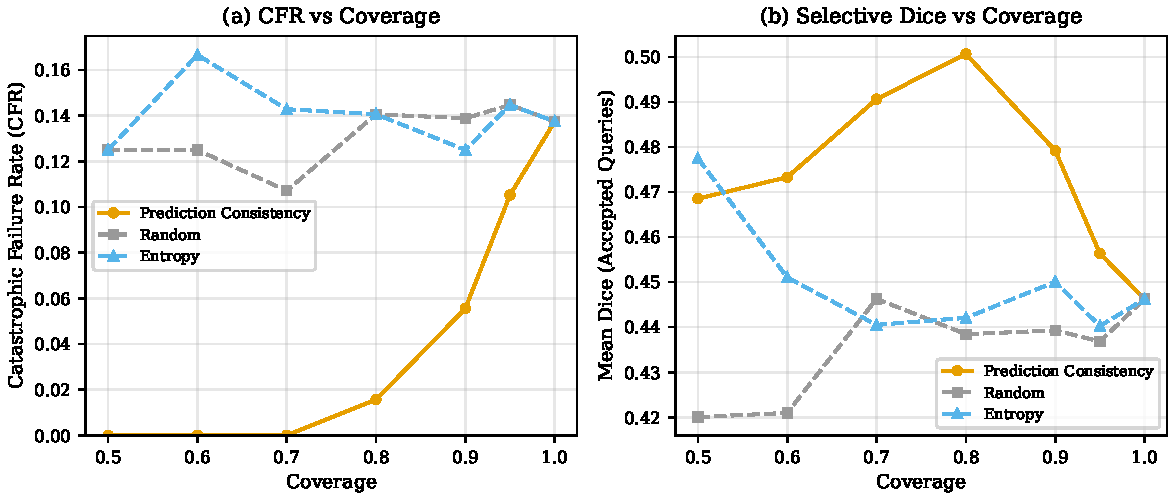
\includegraphics[width=\textwidth]{figures/fig1_risk_coverage_curves.pdf}
\caption{Risk-coverage curves for the primary pipeline (DINOv2-L + SAM-B, 80 queries). 
(a) CFR vs.\ coverage: Prediction consistency substantially reduces CFR across all coverage 
levels. (b) Selective Dice vs.\ coverage: Dice of accepted queries is maintained or improved.}
\label{fig:risk_coverage}
\end{figure}

\begin{figure}[t]
\centering
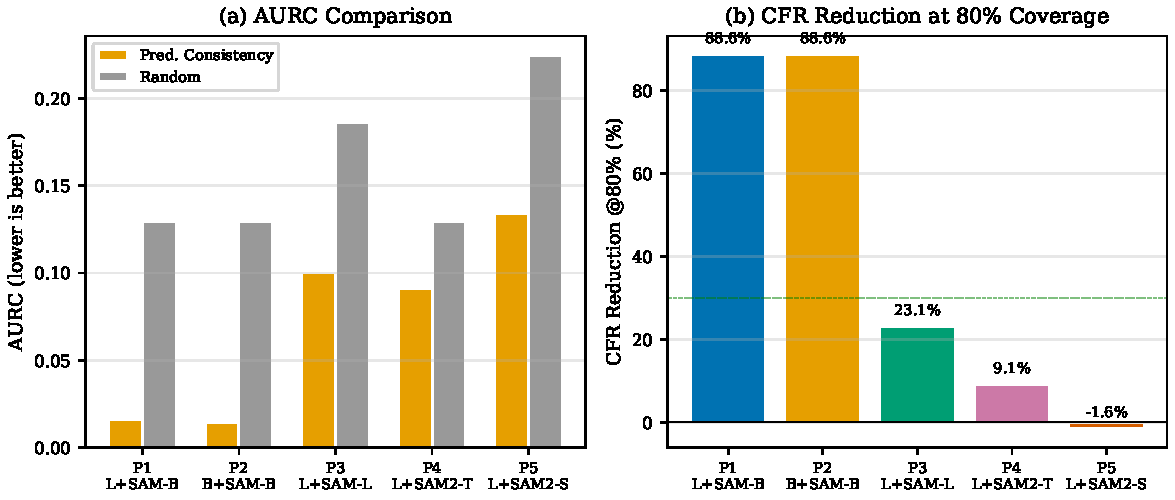
\includegraphics[width=\textwidth]{figures/fig2_cross_pipeline.pdf}
\caption{Cross-pipeline summary. (a) AURC comparison between prediction consistency and 
random ranking. (b) CFR reduction at 80\% coverage. SAM-B pipelines (P1, P2) show the 
strongest effects.}
\label{fig:cross_pipeline}
\end{figure}

\begin{figure}[t]
\centering
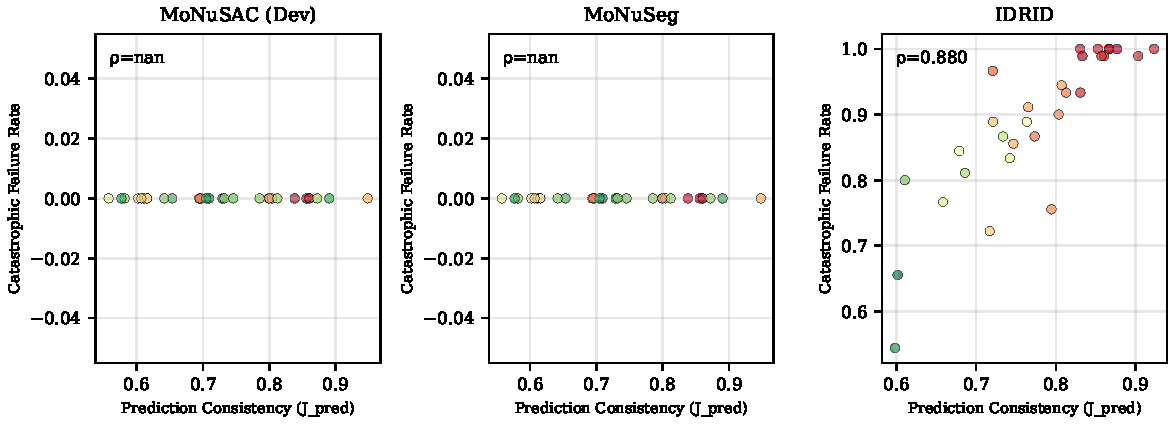
\includegraphics[width=\textwidth]{figures/fig3_cross_dataset_boundary.pdf}
\caption{Cross-dataset boundary analysis. Prediction consistency (x-axis) vs.\ catastrophic 
failure rate (y-axis) per query, colored by mean Dice. Spearman $\rho$ shown for each dataset.}
\label{fig:cross_dataset}
\end{figure}

\begin{figure}[t]
\centering
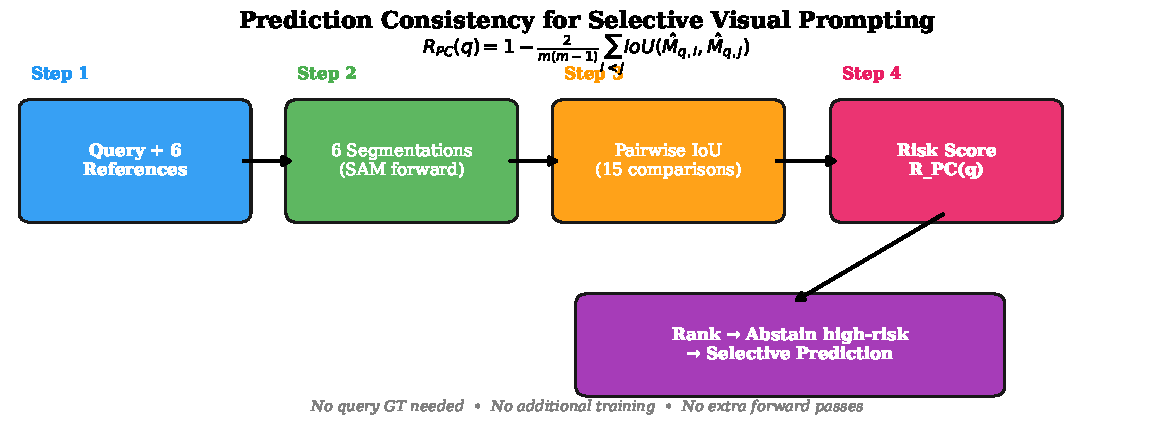
\includegraphics[width=\textwidth]{figures/fig4_method_schematic.pdf}
\caption{Method overview. Prediction consistency requires no query GT, no additional training, 
and no extra forward passes beyond those already performed in multi-reference inference.}
\label{fig:method}
\end{figure}

% ======================================================================
\section{Failure Analysis}

\subsection{When Prediction Consistency Fails}
\textbf{Low base segmentation quality}: When the base segmenter produces consistently poor 
segmentations (e.g., IDRID with Dice=0.098), the pairwise IoU may be consistently low, 
reducing dynamic range. \textbf{Absence of catastrophic failures}: When no catastrophic 
failures exist (e.g., MoNuSeg with CFR=0.0), selective prediction provides no benefit. 
\textbf{Architecturally-limited pipelines}: SAM2-Small produces low-quality segmentations 
and the prediction consistency signal is weaker.

\subsection{When Prediction Consistency Works}
The method is most effective when the base segmenter produces reasonable-quality segmentations, 
there exists a meaningful fraction of high-risk queries, and the references provide sufficient 
variation to reveal inconsistency.

% ======================================================================
\section{Limitations}

\begin{enumerate}[leftmargin=*]
\item \textbf{No Confirmatory Cohort}: Results are based on a development cohort. No fresh, 
independent confirmatory cohort was available. This is an exploratory/benchmark study.
\item \textbf{Pipeline Specificity}: Strongest for SAM-B pipelines; weaker for SAM2-based pipelines.
\item \textbf{Single Task Domain}: Primary evaluation on nuclei segmentation. Cross-dataset 
evaluation on IDRID shows boundary behavior.
\item \textbf{Reference Quality Dependence}: Requires a support set of reference image-mask pairs.
\item \textbf{Multi-Reference Inference Cost}: Requires $m$ forward passes through the segmenter 
(6$\times$ for $m=6$).
\item \textbf{No Absolute Quality Guarantee}: Estimates relative risk within a batch, not absolute quality.
\end{enumerate}

% ======================================================================
\section{Conclusion}

We presented a simple yet effective approach to reliability estimation in multi-reference 
visual prompting. Prediction consistency---the agreement among segmentations from different 
references---serves as a practical, GT-free risk signal. Through systematic evaluation across 
five pipelines and three datasets, we demonstrated effective selective prediction with 88.6\% 
CFR reduction at 80\% coverage. We provided honest analysis of boundary conditions and 
limitations. Future directions include confirmatory evaluation on fresh independent cohorts, 
extension to natural image domains, and integration with model-level uncertainty estimation.

% ======================================================================
\appendix
\section{Appendix}

\subsection{RRN Results}
The Reference Reliability Network (RRN), a learned risk estimator, achieves AUROC=0.573. 
This is below the 0.70 threshold for practical utility. RRN is not recommended as a primary method.

\subsection{Anti-Correlation as Mechanical Artefact}
Corrected $\Delta r$ values are +0.071 (L+SAM-B) and +0.034 (B+SAM-B), indicating the 
anti-correlation is a mechanical artefact rather than a structural property.

\subsection{Full RAMP Component Ablation}
Full RAMP provided no meaningful improvement over simple consensus ($\Delta$Dice = 0.0). 
Removed from main method.

\subsection{Power Analysis}
Bootstrap-based power analysis recommends N=75 queries for confirmatory evaluation, 
with $\ge$10 expected catastrophic events. Current development cohort (N=80) meets this threshold.

\subsection{Reproducibility Checklist}
Code, frozen config, and all hyperparameters are available. Primary pipeline: DINOv2-L + SAM-B. 
Reference count: 6, seed: 42. Query-level statistics with bootstrap CIs. No query GT used in 
risk construction.

\end{document}
